%!TEX root = ../../super_main.tex

\section{Campaign Specification}
\label{sec:campaign_specification}
AndWellness had a concept of campaigns \secref{sec:start_configuration} which we liked. We think we could introduce something similar to their campaigns in this project. Our concept of a campaign and its model will be known as a \textit{campaign specification}, it includes questionnaire specifications, snapshot specifications, and trigger specifications\todo{Overvej om vi skal have triggers med}. The details of our \textit{campaign specification} is further described in this section. This \textit{campaign} model will have to coexist server side and client side in order to enable customers to specify campaigns and participant devices to subscribe to them. The \textit{campaign specification} is a blueprint for how a campaign should be executed on devices. An execution of a campaign should end up with a lot of data which should also be modelled. This data model also coexits on both sides of the system and is described in \secref{sec:snapshot}.

\subsection{Questionnaire Specification Model}
\label{sub:questionnaire_model}
We had come to the conclusion that customers should be able to define questionnaires to be a part of the data collection \secref{sec:human_activity_recognition}. Customers should be able to define one or more separate questions or more generally data inputs which combined should make out a questionnaire model. 
\\\\
Simple boolean yes/no questions can directly be combined to create a discrete amount of labels or classes which can later be used as targets for an AI model but more open inputs, which for instance can be used for regression or as more diverse features, should also be possible. \todo{Overvej om vi når at implementere continuous inputs}
\\\\
A questionnaire specification should be transformable to a format which can be easily be parsed and send from the server to the collecting devices. We have therefore implemented a questionnaire to be Java Parcelable. \todo{Overvej at ændre det her hvis vi gør det til JSON ting i stedet}

\todo[inline]{Overvej om den figur skal opdateres med muligheder for mere advancerede input}
\todo[inline]{ref til figur}
\begin{figure}[!htbp]
	\centering
	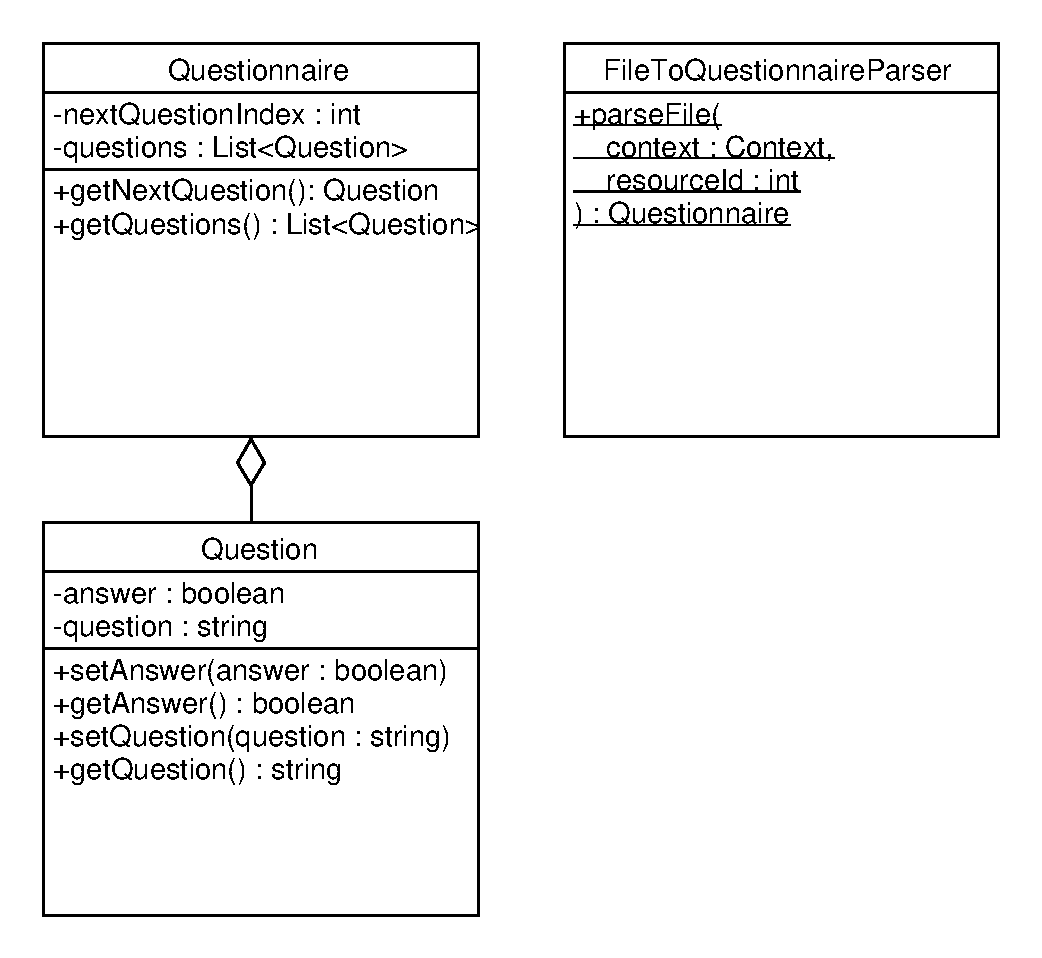
\includegraphics[width=0.6\textwidth]{graphic/data_modeling/questionnaire.pdf}
	\caption{The model of the questionnaires in the system.}
	\label{fig:questionnaire_model}
\end{figure}
\FloatBarrier

\subsection{Sensor Specification Model}
\label{sub:sensor_specification_model}

We need a nested concept or model in the \textit{campaign specification} to able to describe different parameters for the data collection from different sensors. This sensor specification model should include which sensor to sample from, the timings of when to sample data from the given sensor. 


\subsection{Campaign Class Diagram}
\label{sub:campagin_class_diagram}

Questionnaires are not the only source of data and different configurations of the different available sensors should also be customizable for customers. They should be able to specify which data sources they want to include, when they want the data gathered, and how much data they want at a time. 

\todo{Ret figur til - Der vi skal have separeret specification af campaign fra opsamlet data}

\todo[inline]{ref til figur}
\begin{figure}[!htbp]
    \centering
    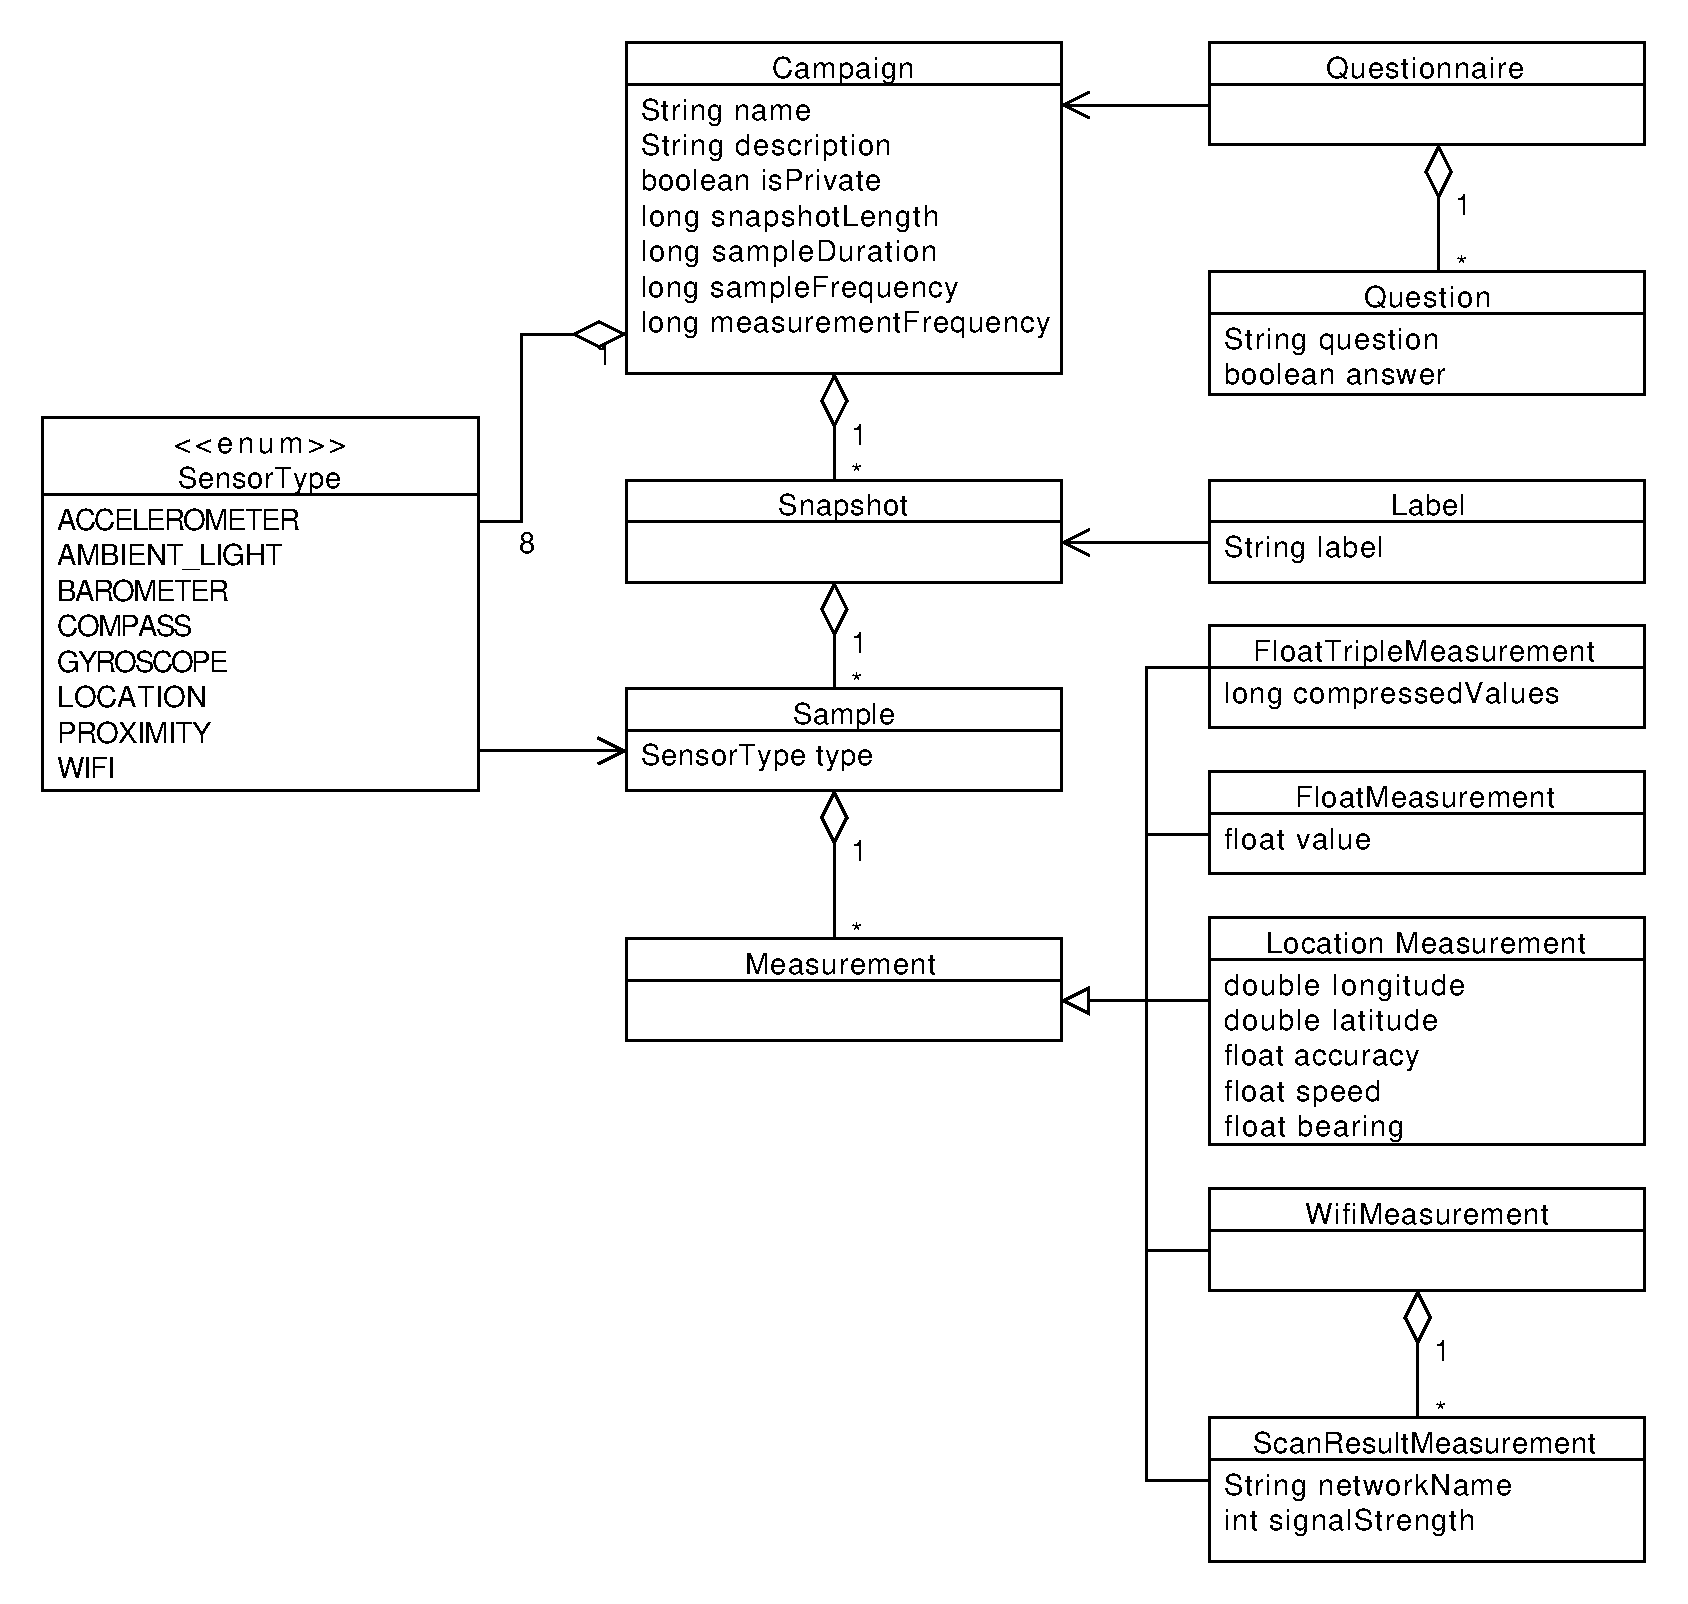
\includegraphics[width=\textwidth]{graphic/data_modeling/model_class_diagram.pdf}
    \caption{Class Diagram of the campaign model.}
    \label{fig:model_class_diagram}
\end{figure}
\FloatBarrier

